\documentclass{article}

\usepackage{listings}
\usepackage{float}
\usepackage[twoside]{fancyhdr}
\usepackage{hyperref}
\usepackage{lastpage}
\usepackage{courier}
\usepackage{graphicx}
\usepackage[dvipsnames]{xcolor}

\lstset {
	basicstyle=\small\ttfamily,
	breaklines=true
}

\renewcommand{\labelitemi}{$\diamond$}

\pagestyle{fancy}
\pagenumbering{roman}

\fancyhead[LE,RO]{\textsc{\rightmark}}
\fancyhead[RE,LO]{}
\fancyfoot[RE,LO]{Page \thepage\ of \pageref{LastPage}}
\fancyfoot[LE,RO]{}
\fancyfoot[C]{}

\renewcommand{\sectionmark}[1]{\markright{#1}{}}


\renewcommand{\headrulewidth}{2pt}
\renewcommand{\footrulewidth}{2pt}


\begin{document}
	\begin{titlepage}
		\begin{center}
			\Huge\textsc{Beginning with programming in Arduino}
			
			\vfill
			
			\huge\textbf{27 October 2024}
			
			\vfill
			
			\Large\textsc{Archived By}\\
			\Large\textbf{b33tr00t-444}
		\end{center}
	\end{titlepage}

\pagestyle{plain}

\tableofcontents

\pagebreak

\listoffigures

\pagebreak

\lstlistoflistings

\pagebreak

\section{The Basics}
\pagestyle{fancy}
\setcounter{page}{1}
\pagenumbering{arabic}
\paragraph{}

\begin{itemize}
	\item Format of code in for Arduino:
	
	\begin{lstlisting}[frame=TlbR, caption=Arduino code format]
void setup() {
}

void loop() {
}
	\end{lstlisting}

Commands put inside of \lstinline|setup()| are executed once. This function is used to `setup' the arduino board. Commands that we want to run over and over again are put inside of the \lstinline|loop()| function.

\item Now, I am using \href{https://arduino.github.io/arduino-cli/1.0/}{\textcolor{Blue}{Arduino CLI}} here. To see the list of connected boards use the following command:

\begin{lstlisting}[frame=tLBr, caption=Viewing the list of connected boards]
$ arduino-cli board list
\end{lstlisting}

This will display a list of connected boards with their name, FQBN(Fully Qualified Board Name), port, etc. In my case, however, it's showing the following:

\begin{figure}[H]
	\centering
	\fbox{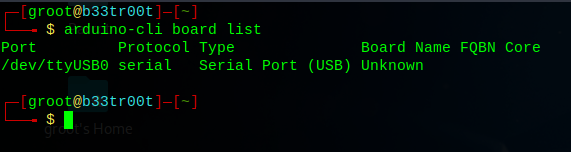
\includegraphics[width=100mm]{images/boardList.png}}
	\caption{Listing the connected boards}
	\label{fig:fig1}
\end{figure}

Here, it doesn't show my board's name, instead, it shows `Unknown'. I know that my board is an Arduino Uno, so I will do a \lstinline|core search| for my board by using the following command:

\begin{lstlisting}[frame=tLBr, caption=Search for my board]
$ arduino-cli core search uno
\end{lstlisting}

\pagebreak
This will generate the following output:

\begin{figure}[H]
	\centering
	\fbox{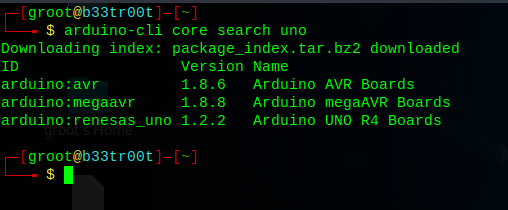
\includegraphics[width=100mm]{images/searchingUno.png}}
	\caption{Searching my board}
	\label{fig:fig2}
\end{figure}

Those names mentioned below the \lstinline|ID| column are the names of the platform needed for the board, the correct platform needs to be installed to be able to use the board. Based on what I have found (by googling), I need to install the \lstinline|arduino:avr| platform for my UNO.

\item To install the required platform, just use the following command:

\begin{lstlisting}[frame=tLBr, caption=Installing the platform]
$ arduino-cli core install arduino:avr
\end{lstlisting}

\begin{figure}[H]
	\centering
	\fbox{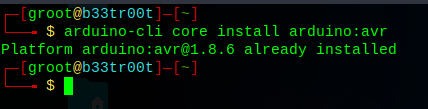
\includegraphics[width=100mm]{images/installingPlatform.png}}
	\caption{Installing the required platform}
	\label{fig:fig3}
\end{figure}

In my case, it has already been installed for my board (because I had already installed it earlier and this was done for illustration purposes).

\item Once it's installed, we need to know the FQBN for our board and for that we need to list all the boards but this time it's a different command:

\begin{lstlisting}[frame=tLBr, caption=Listing all the boards]
	$ arduino-cli board listall
\end{lstlisting}

\pagebreak

This produces the following:

\begin{figure}[H]
	\centering
	\fbox{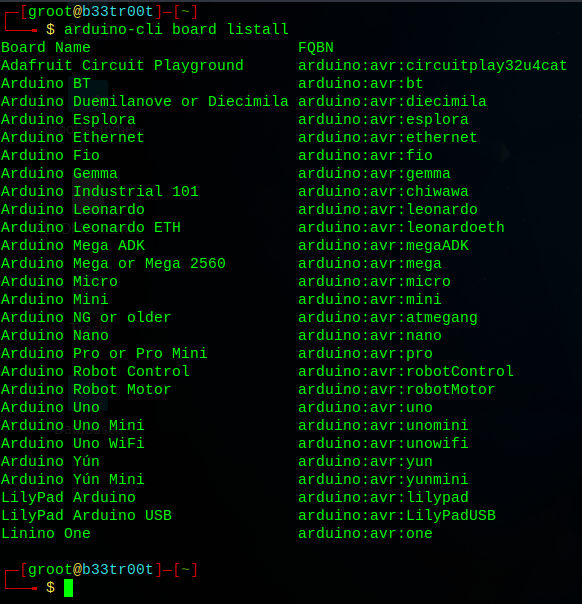
\includegraphics[width=100mm]{images/listingAllBoards.png}}
	\caption{Listing all the boards}
	\label{fig:fig4}
\end{figure}

As seen from the image, the FQBN for Arduino UNO is mentioned alongside with its Board Name. Now, I can use this FQBN for compiling and uploading my sketch to my board.
\end{itemize}

\pagebreak

\section{Writing my first program}
\paragraph{}

\begin{itemize}
	\item The pin 13 of the arduino is connected to a LED (labelled as \lstinline|L| on the board).
	\item My first program in Arduino:
	
	\begin{lstlisting}[frame=TlbR, caption=First program, label=lst:lst1]
void setup() {
	pinMode(13, OUTPUT);
}

void loop() {
	digitalWrite(13, HIGH);
}

	\end{lstlisting}

	\item To compile this program in arduino CLI, we compile it using the following command:
	
	\begin{lstlisting}[frame=tLBr, caption=Compiling an arduino program]
$ arduino-cli compile -b arduino:avr:uno /home/groot/arduino/programs/first/first1/first1.ino
	\end{lstlisting}

	\item After compiling the sketch, we need to upload it using the following command:
	
	\begin{lstlisting}[frame=tLBr, caption=Uploading the sketch]
$ arduino-cli upload -p /dev/ttyUSB0 -b arduino:avr:uno /home/groot/arduino/programs/first/first1/first1.ino
	\end{lstlisting}

	\item After uploading it to the board, the LED will be turned on.
	
	\item Basically in \textcolor{Red}{Listing \ref{lst:lst1}} in the function \lstinline|pinMode()| I have added two parameters, the first is the \emph{pin number} and the second is whether that pin should be treated as an \emph{input} or an \emph{output}. Since I am going to turn it on/off (it's going to output its state), so it's set to \lstinline|OUTPUT|. Next, in the function \lstinline|loop()|, I have put the line \lstinline|digitalWrite(13, HIGH);| which basically means that it's going turn the LED (\lstinline|13|) on (\lstinline|HIGH|) and this command is going to repeat over and over again because that's what \lstinline|loop()| does.
	
	\newpage
	
	\item Here's a modified version of \textcolor{Red}{Listing \ref{lst:lst1}}:
	
	\begin{lstlisting}[frame=TlbR, caption=Blinking LED, label=lst:lst2]
void setup() {
	pinMode(13, OUTPUT);
}

void loop() {
	digitalWrite(13, HIGH);
	delay(1000);
	digitalWrite(13, LOW);
	delay(1000);
}

	\end{lstlisting}
	
	\item I have added a another \lstinline|digitalWrite()| that turns the LED (\lstinline|13|) off (\lstinline|LOW|).
	
	\item The \lstinline|delay(1000)| function pauses the program for a $1000$ milliseconds (that $1$ second).
\end{itemize}

\pagebreak

\section{Programs}
\paragraph{}

\begin{itemize}
	\item \url{https://github.com/b33tr00t-444/arduino/tree/arduinoFun/programs/first/first1}
	\item \url{https://github.com/b33tr00t-444/arduino/tree/arduinoFun/programs/first/first2}
	\item \url{https://github.com/b33tr00t-444/arduino/tree/arduinoFun/programs/first/first3}
	\item \url{https://github.com/b33tr00t-444/arduino/tree/arduinoFun/programs/first/assignment}
\end{itemize}

\end{document}